\documentclass{article}
\usepackage{placeins}
\usepackage{siunitx}
\usepackage{graphicx}

\begin{document}
\begin{titlepage}
	\centering
	\vspace{2.5cm}
	\vspace{1cm}
	{\huge Experiment 8 \par}
	{\LARGE MOS Transistors as Switches and Amplifiers \par}
	{\Large EECS 170A - Lab Bench \#1 \par}
	{\Large \today \par}
	\vspace{1cm}
	{\large Roman Parise (59611417) \par}
	{\large Krishan Solanki (38154673) \par}
	{\large Jason Wang (42873192) \par}
	\vspace{1cm}
\end{titlepage}
\section{Procedure}
The objective of this lab is to design a transistor inverter and observe both the switching and amplifier characteristics of MOSFETs. For the first circuit, the switching behavior of a MOSFET is observed. A circuit with multiple components is built and a voltage pulse is given to the transistor to observe the output voltage signal. The input pulse signal is increased so both the turn-on and turn-off transients are observed and the time delay, rise time, and fall time are measured. Next, the circuit for the MOSFET Amplifier is built. The bias voltage is measured without connecting the input source to the amplifier, which should be half of the DC power supply. After measuring, apply an input signal at 10kHz frequency to display both the input and output voltage signal (sinusoidal). The input voltage is increased until the output voltage starts to clamp. The gain is then measured. The upper cutoff frequency is measured along with voltage gain at the certain frequency. Lastly, the cutoff frequency is tested while observing the output after setting the function generator to square wave input. \\

\section{Results and Analysis}
\subsection{Inverting Characteristics of the MOSFET}
The BJT inverter circuit yields an expected output given a periodic square input signal. As expected, the $10$\si{\kilo\hertz} input signal is essentially inverted by the inverter with slight delay and ramping due to the recombination of excess carriers during the BJT's transition from saturation operation to cutoff operation and vice versa. The large delay times or slow switching behavior characteristic of the BJT makes the BJT inverter circuit unusable in high frequency RF applications. 

\subsection{Amplifying Characteristics of the MOSFET}
The inverter circuit constructed in Figure \ref{fig:mos_inverter} is also called a common-source amplifier and the amplification characteristics of the circuit is explored in this experiment by analyzing its frequency response.

For this portion of the experiment the MOSFET must always be operating in saturation mode, meaning the condition in Equation \ref{eq:sat_mode} must be satisfied. Because a sinusoidal wave is used as the input signal, a DC offset must be applied so that $V_{GD} < V_{Th} = 2$\si{\volt} for the entire amplitude range of the sinusoidal input. 

The amplifier's input signal is chosen to have $200$\si{\milli\volt}pp with a $2.5$\si{\volt}dc offset and a frequency of $10$\si{\kilo\hertz} because at this setting it is observed that the entire amplitude range of the input just lies within the saturation region. Clipping is observed in the output signal when the amplitude of the input signal is increased to $250$\si{\milli\volt}pp. This occurs because a portion of the positive cycle of the input signal now lies outside the saturation region and crosses over to the triode region. 

\FloatBarrier
\begin{figure}[h!]
	\centering
	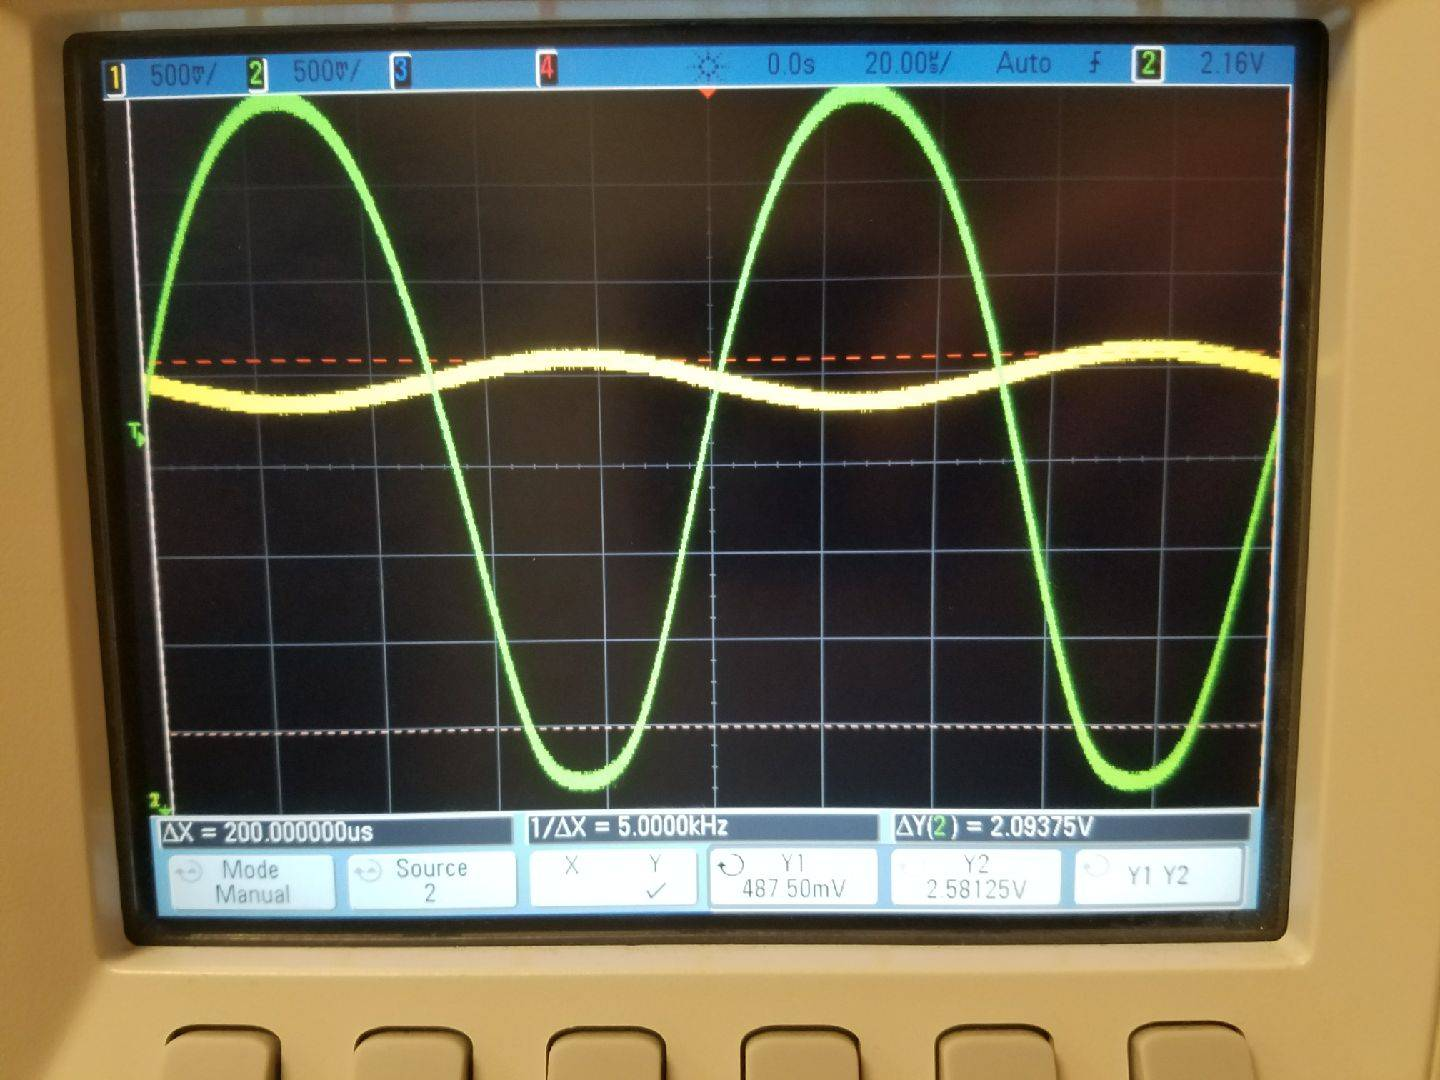
\includegraphics[scale=0.25]{../images/amplifier_clamping.jpeg}
	\caption{Common-Source Amplifier $10$\si{\kilo\hertz} Distortions}
	\label{fig:amplifier_clipping}
\end{figure}
\FloatBarrier

Like the common-base amplifier observed in the previous experiment, the common-source amplifier is also a non-ideal amplifier due to capacitive effects. Consider the physical structure of the MOSFET, more specifically the nMOS:

\FloatBarrier
\begin{figure}[h!]
	\centering
	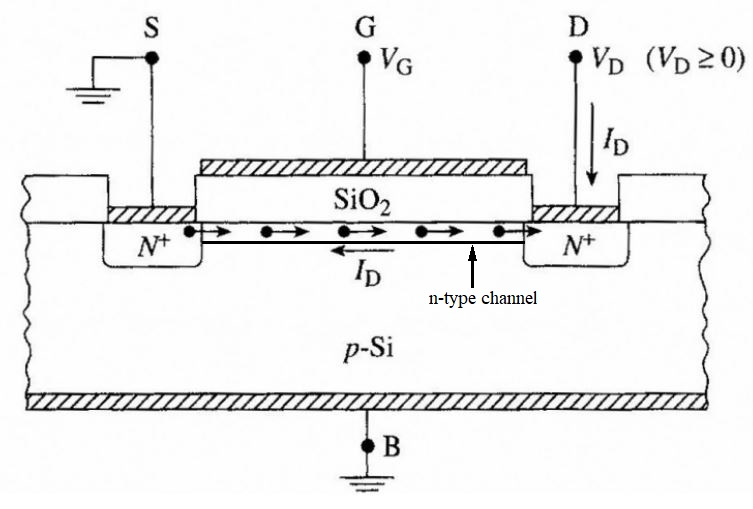
\includegraphics[scale=0.9]{../images/nmos_structure.JPG}
	\caption{Physical Structure of MOSFET}
	\label{fig:nmos_structure}
\end{figure}
\FloatBarrier

There is capacitance between the gate to source ($C_{gs}$) and gate to drain ($C_{gd}$) due to two reasons: the overlap of the metal gate electrode and the wells of n+ semiconductor material at the source and drain, and the close proximity of the metal gate electrode and the induced n-type channel. There is also junction capacitance between the n+ drain to p-type substrate body ($C_{db}$) and n+ source to p-type substrate body ($C_{sb}$) (\ref{capacitive_effects}). The equivalent circuit is given in the following model:

\FloatBarrier
\begin{figure}[h!]
	\centering
	\caption{MOSFET High Frequency Small Signal Model}
	\label{fig:mos_amp}
	\begin{circuitikz}
		\draw
		( 0 , 0 ) node[ nmos ] (my_nmos) {}
		
		% Gate
		(my_nmos.G) to [ short ] ++( -3 , 0 ) coordinate(g_out)
		(g_out) to [ sV , v<=$V_{in}$ ] ++( 0 , -3 ) coordinate(gnd_1)
		(gnd_1) node[ ground ] (my_gnd_1) {}
		
		% Drain
		(my_nmos.D) to ++(0,1) coordinate(r)
		(r) to [ R={$300\Omega$} ] ++( 0 , 2 ) coordinate(vcc)
		(vcc) to [ battery , v<=$V_{dd}\rightarrow5V$ ] ++( 3 , 0 ) coordinate(gnd_3)
		(gnd_3) node[ ground ] (my_gnd_3) {}
		
		% Source
		(my_nmos.S) to ++(0,-1) node[ ground ] (my_e_gnd) {}
		
		% Parasitic Caps
		(r) to [ C={$C_{db}$} ] ++( 2 , 0 ) coordinate(cdb)
		(cdb) node[ ground ] (my_gnd_4) {}
		(my_e_gnd) to [ C={$C_{sb}$} ] ++( 2 , 0 ) coordinate(csb)
		(csb) node[ ground ] (my_gnd_5) {}
		(r) to [ C, l_={$C_{gd}$} ] (g_out) 
		(my_e_gnd) to [ C={$C_{gs}$} ] (g_out) 
		
		;
	\end{circuitikz}
\end{figure}
\FloatBarrier

At low frequencies, the capacitors in the circuit above are essentially open circuits and thus the amplifier exhibits ideal behavior and maximum gain. However, when the frequency of the input is sufficiently high, the capacitors begin to short the path from the drain to ground, effectively decreasing the amplitude of the output voltage. Increasing the frequency of the input signal will drop the amplitude of the output signal further until $V_{out} = 0$\si{\volt}. This also causes the gain in \si{\decibel} of the amplifier to drop as gain is given by $20log(\frac{V_{out}}{V_{in}})$. 

At 10\si{\kilo\hertz}, the input voltage value of 200\si{\milli\volt}pp corresponds to an output voltage value of $3.3$\si{\volt}pp. $\frac{V_{out}}{V_{in}}$ at 10\si{\kilo\hertz} is calculated to be $16.5$ and a gain in \si{\decibel} of $24.3$\si{\decibel}. This gain value corresponds with the maximum gain because parasitic capacitances are still regarded as open circuits. The parasitic capacitances will then decrease the gain of the amplifier at high frequencies and a cutoff frequency, $f_c$, can be found when the gain in \si{\decibel} is a value that is $3$\si{\decibel} less than the maximum value or when the $\frac{V_{out}}{V_{in}}$ ratio is less than the maximum value by a factor of $\sqrt{2}$. The cutoff should then occur when $\frac{V_{out}}{V_{in}} = \frac{16.5}{\sqrt{2}} = 11.7$ which corresponds to a gain in \si{\decibel} of $21.3$\si{\decibel}. Using the condition above, $f_c$ is observed to be approximately $3.6$\si{\mega\hertz}.

\FloatBarrier
\begin{table}[h!]
	\centering
	\caption{Common-Source Amplifier Frequency Response}
	\label{tab:amplifier_freq}
	\csvautotabular{../tables/amplifier_freq.csv}
\end{table}
\FloatBarrier

A square wave with frequency of $f_c = 3.6$\si{\mega\hertz} is then set as the input signal to observe distortions in the output waveform. Two duty cycles for the square input are used for the observation: $20\%$ and $50\%$. The two duty cycles give the following waveforms:

\FloatBarrier
\begin{figure}[h!]
	\centering
	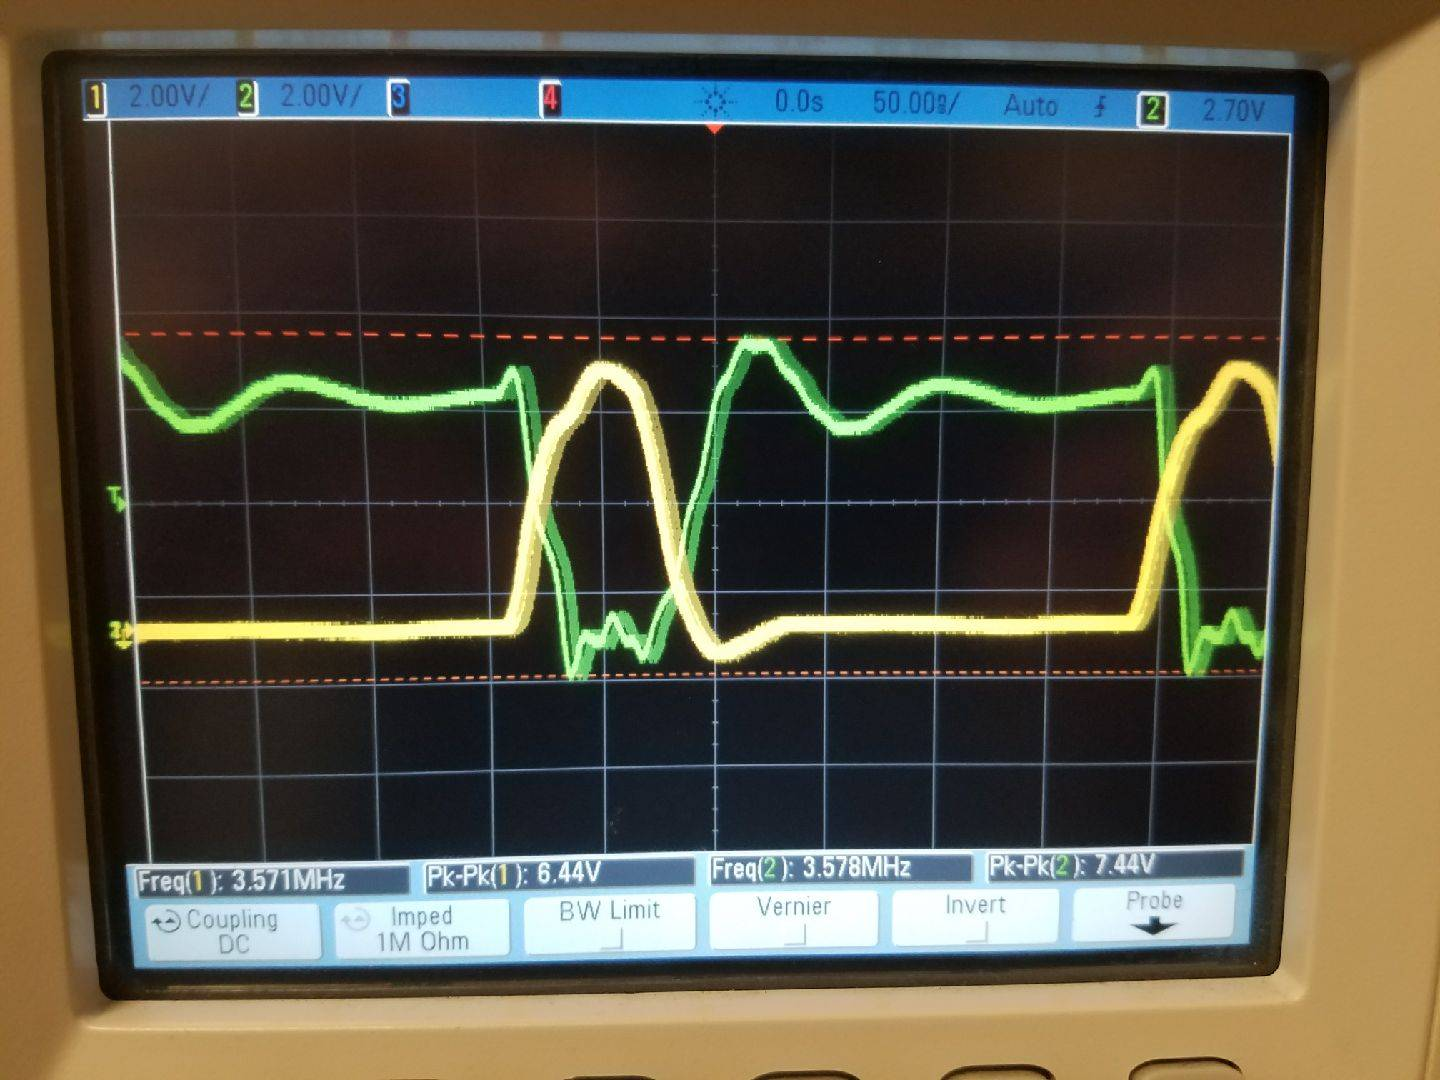
\includegraphics[scale=0.25]{../images/amplifier_20.jpeg}
	\caption{Common-Source Amplifier Square Wave Response $20\%$ Duty Cycle}
	\label{fig:amplifier_20}
\end{figure}
\FloatBarrier

\FloatBarrier
\begin{figure}[h!]
	\centering
	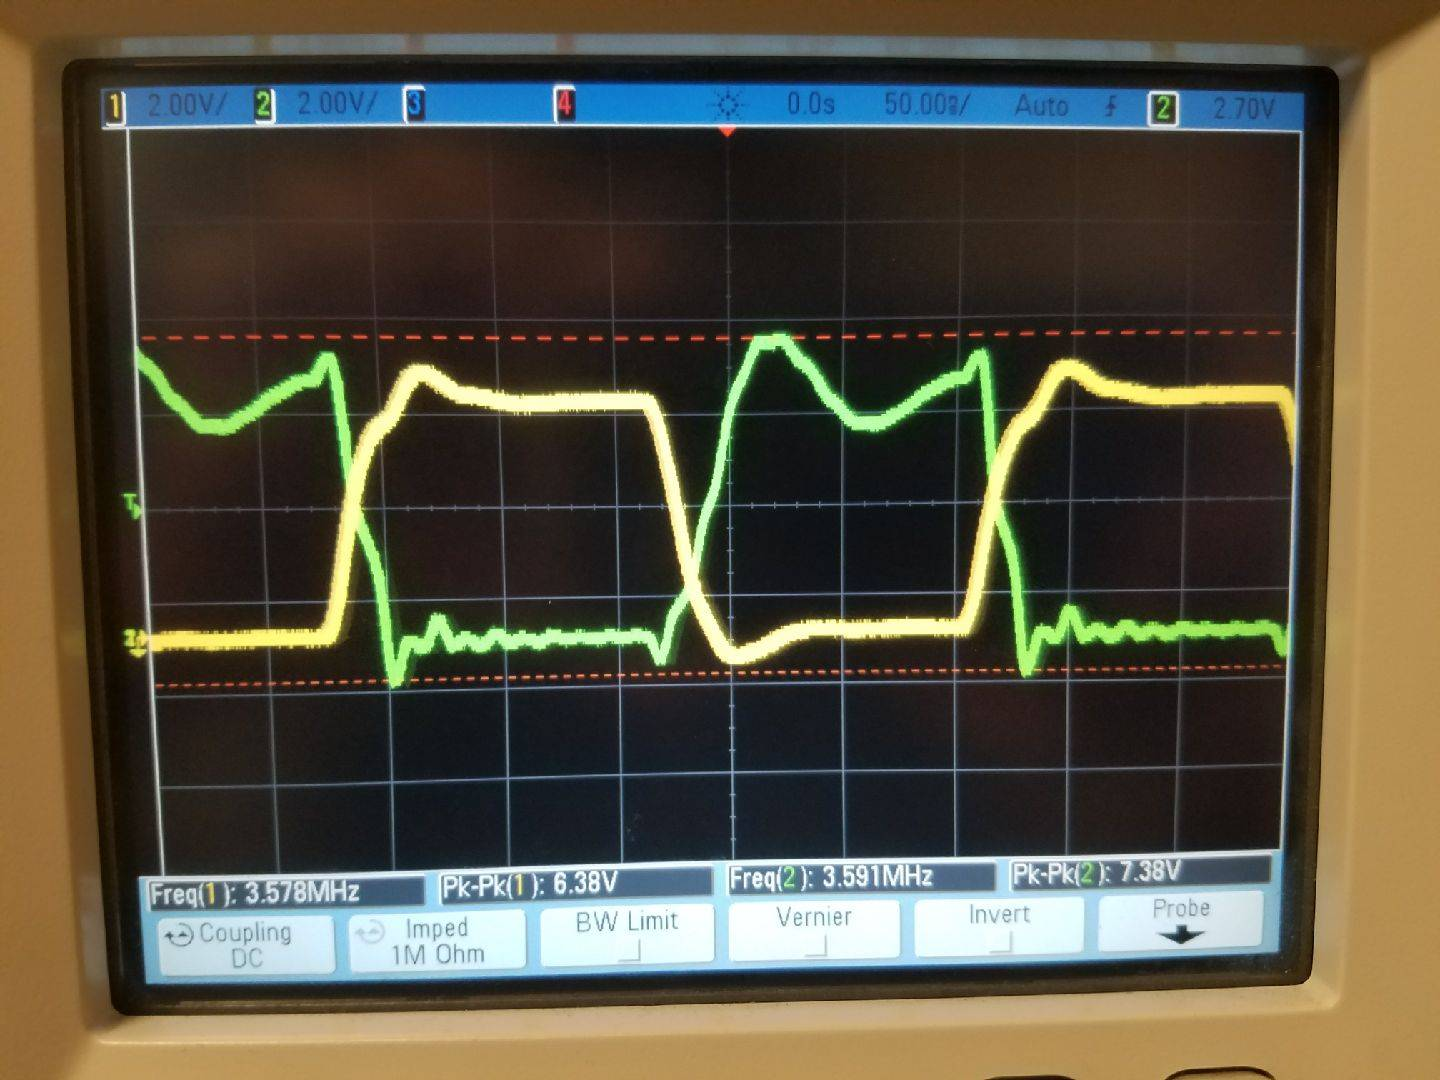
\includegraphics[scale=0.25]{../images/amplifier_50.jpeg}
	\caption{Common-Source Amplifier Square Wave Response $50\%$ Duty Cycle}
	\label{fig:amplifier_50}
\end{figure}
\FloatBarrier

For both the $20\%$ and $50\%$ duty cycle square inputs, the input and output signals have very noticeable distortions due to second-order effects. However, if the distortion is ignored, the output signal still resembles an inversion of the input signal. This is because at 3.6\si{\mega\hertz}, the period of the wave is $278$\si{\nano\second} which is still significantly higher than the delay times, rise time, and fall time found in the inverter experiment. This means that for both duty cycles, the output voltage still has sufficient time to fully develop.
\section{Discussion}
\subsection{Inverting Characteristics of the MOSFET}
The MOSFET exhibits the inverting capabilities predicted by theory. It also switches at a much faster rate than the bipolar-junction transistor (BJT). An equivalent BJT circuit would have rise and fall times as well as delays in the \si{\micro\second} range, whereas the MOSFET's are in the \si{\nano\second} range. Moreover, the MOSFET operates in saturation when the input is high and cutoff when the input is low, a desired characteristic of the circuit. Given the measured data, it is clear that the output voltage $V_{out}$ takes longer to transition from low to high than it does to transition from high to low. Furthermore, the MOSFET is unable to operate at high frequencies, such as $3$\si{\giga\hertz}, inasmuch as it is limited by its state transition delays.

\subsection{Amplifying Characteristics of the MOSFET}
The common-source amplifier which utilizes the MOSFET has a significantly higher cutoff frequency than the common-emitter amplifier which utilizes the BJT. The common-emitter amplifier would have its cutoff frequency around the order of magnitude of $~100$\si{\kilo\hertz} while the common-source amplifier is found to have its cutoff frequency in the \si{\mega\hertz} range. However, noticeable second-order distortion is observed in input and output signals that approach or exceed the cutoff frequency. This distortion however, is not due to delay times as it is observed that inversion and amplification still occurs at an adequately fast pace around the cutoff frequency. For the common-emitter amplifier, second-order effects are not seen near the cutoff frequency, but switching time is too slow for voltages to fully develop. As a result, the advantages and disadvantages of the MOSFET and BJT are made more clear.
\section{References}
1. \url{http://aries.ucsd.edu/NAJMABADI/CLASS/ECE102/12-F/NOTES/ECE102_F12-LecSet-8.pdf} \\
\end{document}
